\documentclass[a4paper, 12pt, spanish]{scrartcl}
\usepackage[utf8]{inputenc}
\usepackage[T1]{fontenc}
\usepackage[spanish]{babel}

\renewcommand{\labelitemi}{$\bullet$}
\renewcommand{\labelitemii}{$\bullet$}
\renewcommand{\labelitemiii}{$\bullet$}

\usepackage{caption}
\usepackage{csquotes}
\usepackage{graphicx}

\usepackage[none]{hyphenat}
\usepackage{lmodern}
\usepackage{microtype}

\newcommand{\todo}[1]{\noindent\textcolor{red}{\textbf{Pendiente: }#1}}
\newcommand{\todoref}[1]{\noindent\textcolor{cyan}{\textbf{Referencia: }#1}}
\newcommand{\redactar}[1]{\noindent\textcolor{blue}{\bfseries #1}}

% _ escaping
\catcode`\_=12

% Lean3 formatting
\usepackage{amssymb}
\usepackage{amsthm}
\usepackage{upgreek}
\usepackage{listings}
\usepackage{xcolor}
\definecolor{backcolor}{rgb}{0.9, 0.9, 0.9}   % grey
\definecolor{keywordcolor}{rgb}{0.7, 0.1, 0.1}   % red
\definecolor{commentcolor}{rgb}{0.4, 0.4, 0.4}   % grey
\definecolor{symbolcolor}{rgb}{0.0, 0.1, 0.6}    % blue
\definecolor{sortcolor}{rgb}{0.1, 0.5, 0.1}      % green
\definecolor{errorcolor}{rgb}{1, 0, 0}           % bright red
\definecolor{stringcolor}{rgb}{0.5, 0.3, 0.2}    % brown
\definecolor{tacticcolor}{rgb}{0.0, 0.1, 0.6}

\renewcommand{\lstlistingname}{Listado}

\def\lstlanguagefiles{lstlean.tex}

\lstdefinestyle{leanBase}{
	language=lean,
	aboveskip=1em,
	belowskip=.5em,
}

\lstdefinestyle{leanSimple}{
	style=leanBase,
	frame=trlb,
	framesep=10pt,
	rulecolor=\color{gray},
	basicstyle=\fontsize{10}{11}\selectfont\ttfamily,
	xleftmargin=-.75cm,
	xrightmargin=-.75cm,
	aboveskip=1em,
	belowskip=.5em,
	% framexleftmargin=1em,
	% framexrightmargin=1em,
}
\lstdefinestyle{leanFull}{
	style=leanSimple,
	numbers=left,
	% numbersep=5pt,
	xleftmargin=0cm,
	framexleftmargin=.75cm,
	numberstyle=\scriptsize\ttfamily\color{gray},
	% belowskip=-.5em,
	% backgroundcolor=\color{backcolor}, % background color
}

\lstset{style=leanSimple}

\newcommand{\lstleanfull}[3]{
	\lstinputlisting[
		style=leanFull,
		firstnumber=#2,
		firstline=#2,
		lastline=#3,
		title={\ttfamily \footnotesize src/#1}
	]{../src/#1}
}

\newtheorem{prop}{Proposición}
\newtheorem{tma}{Teorema}
\newtheoremstyle{defin}{14.0pt plus 2.0pt minus 4.0pt}{0mm}{}{}{\bfseries}{.}{.5em}{}
\theoremstyle{defin}
\newtheorem*{defin*}{Definición}

\def\theaxsection{}
\newcommand{\setaxsection}[1]{\def\theaxsection{#1}\setcounter{ax}{0}}

\newtheoremstyle{axstyle}{\topsep}{\topsep}{\itshape}{0pt}{\bfseries}{.}{ }
{\thmname{#1} \theaxsection\thmnumber{#2}\textnormal{\thmnote{ (#3)}}}
\theoremstyle{axstyle}
\newtheorem{ax}{Axioma}
\newtheoremstyle{axbstyle}{\topsep}{\topsep}{\itshape}{0pt}{\bfseries}{.}{ }
{\thmname{#1}\thmnote{ #3}}
\theoremstyle{axbstyle}
\newtheorem{axb}{Axioma}




% \usepackage{lstautogobble}

\setlength\parindent{0pt}
\setlength\parskip{1em plus 0.1em minus 0.2em}
\addtolength{\skip\footins}{.5em}

\usepackage{dirtree}

\usepackage[colorlinks=true, linktocpage=true, citecolor=red, linkcolor=blue]{hyperref}

\setcounter{tocdepth}{2}


% \usepackage{sectsty} % Comentado porque generaba warning https://tex.stackexchange.com/a/310968

\newcommand{\emptypage}{\newpage\null\thispagestyle{empty}\newpage}
\usepackage[margin=3cm]{geometry}


\renewenvironment{abstract}[1][Resumen]{
	\thispagestyle{empty}
	\begin{center}
		\textbf{#1}
	\end{center}
}{\vspace*{1cm}}

% \usepackage{titlesec}
% \titleformat{\section} {\Large\bfseries}{\thesection.}{0.5em}{}
% \titleformat{\subsection}{\large\bfseries}{\thesubsection.}{0.5em}{}
% \titleformat{\subsubsection}{\normalfont\bfseries}{\thesubsubsection.}{0.5em}{}
% \titlespacing*{\subsubsection}{0pt}{.3em plus 0.1em minus 0.1em}{.05em plus 0.1em minus 0.1em}
% \titlespacing{\paragraph}{0pt}{0.5\baselineskip}{1em}


\usepackage[citestyle=numeric,bibstyle=numeric,sorting=none]{biblatex}

\addbibresource{referencias.bib}

\begin{document}

% Estilo de portada inspirado en https://github.com/guillegran/TFGMates
\begin{titlepage}
	\begin{minipage}{.5\textwidth}
		\Large Trabajo de Fin de Grado
	\end{minipage}
	\begin{minipage}{0.5\textwidth}
		\hfill
		
\includegraphics[height=1.5cm]{imgs/UCM}
	\end{minipage}
	\vfill
	\begin{center}

		{\LARGE Formalización de las matemáticas con Lean.\\[.6em]
			Un caso de estudio: Geometría euclídea plana.}

		\vspace*{.5cm}

		{\large\normalfont Adrián Lattes Grassi}

		\vspace*{.3cm} {\large Septiembre de 2023}
	\end{center}
	\vfill{\Large\noindent Facultad de Ciencias Matemáticas.\\[.6em]
		Trabajo dirigido por Jorge Carmona Ruber.}
\end{titlepage}
% \emptypage

\begin{abstract}
	Este trabajo explora el uso del asistente de demostración Lean, un
	lenguaje que implementa una teoría de tipos, el
	\textit{Cálculo de construcciones inductivas}, utilizando la axiomática de
	Hilbert de la geometría euclídea como guía motivadora para el
	aprendizaje.

	Comentamos aspectos generales de la formalización de matemáticas asistida
	por computadoras, sus aplicaciones y ventajas; se introducen conceptos
	básicos del funcionamiento de Lean; se analiza el trabajo de
	formalización realizado; y se concluye proponiendo una línea de continuación
	del trabajo.
\end{abstract}

\begin{abstract}[Abstract]
	This paper explores the use of the Lean proof assistant, a language that
	implements a type theory, the \textit{Calculus of Inductive Constructions},
	using Hilbert's axiomatics of Euclidean geometry as a motivating guide for
	learning.

	We discuss the general aspects of the computer-assisted formalization of
	mathematics, its applications and advantages; we also introduce basic
	concepts of Lean operation; we analyze the formalization work carried out;
	and we conclude by proposing a line of continuation of the work.

\end{abstract}

\newpage











\tableofcontents
\newpage

\section{Objetivos y metodología}

El objetivo principal de este trabajo es aprender los fundamentos del lenguaje
de programación y asistente de demostración Lean. Sin entrar en
detalles sobre cómo funciona y la implementación del lenguaje, nos hemos
propuesto aprender a utilizarlo como podría usarlo un estudiante o investigador de
matemáticas. Es decir, formalizando resultados matemáticos.

Para esto hemos elegido la geometría euclídea plana, en particular la
axiomatización de David Hilbert realizada a inicios del siglo pasado.
La idea es que esta teoría sirva de guión para formalizar resultados y durante
el proceso de formalización de axiomas y proposiciones aprender las
características y nociones necesarias de Lean.

Otro objetivo más ambicioso, que trasciende las posibilidades de este trabajo,
es el de formalizar la independencia del \textit{axioma de las paralelas} del
resto de axiomas de la geometría. Aún no teniendo el tiempo suficiente para
abordar esta tarea, hemos propuesto una formalización del enunciado de la
independencia y propuesto un plan de trabajo para formalizar su demostración.

Antes de poder emprender el trabajo de formalización de resultados geométricos
ha sido necesario obtener unos conocimientos de base de Lean. Al abordar esta
tarea, en la que aprendimos a expresar y demostrar resultados elementales de
lógica proposicional, a trabajar con estructuras algebraicas y exploramos
ciertas características del lenguaje, las principales referencias han sido los
materiales del curso de Kevin Buzzard, \textit{Formalising
	mathematics}~\cite{buzzardFormalisingMathematicsFormalising}, y el manual
oficial, \textit{Theorem proving in Lean}~\cite{avigadLeanTheoremProver}.

Los materiales del curso, que incluyen ejercicios prácticos, explicaciones
teóricas y soluciones a los ejercicios en formato vídeo han sido especialmente
útiles en este proceso de aprendizaje.

Durante el mes de febrero de 2023 tuvimos la oportunidad de participar en el
curso de doctorado sobre \textit{Formalización de matemáticas en Lean},
impartido por María Inés de Frutos~\cite{defrutosFormalizacionMatematicasLean}.
Asistir a este curso nos permitió afianzar los conocimientos que estábamos
adquiriendo y contrastar dudas o distintas formas de resolver los problemas con
la profesora y los demás participantes del curso.

Para tener un entendimiento a nivel intuitivo de los conceptos necesarios de
teoría de tipos se ha estudiado el primer capítulo del libro \textit{Homotopy
	Type Theory}~\cite{HomotopyTypeTheory} en el que se introducen conceptos de
teoría de tipos y se mencionan sus relaciones con la lógica.

En paralelo a este aprendizaje del lenguaje y herramientas de Lean iniciamos el
estudio de la geometría de Hilbert, apoyándonos principalmente en los libros de
texto de Hartshorne~\cite{hartshorneGeometryEuclid2000} y
Greenberg~\cite{greenbergEuclideanNonEuclideanGeometries1993}, y realizando
alguna consulta al texto original de Hilbert~\cite{hilbertFoundationsGeometry1950},
para conocer cómo fueron formulados originalmente los axiomas, definiciones y
teoremas de la teoría.

Una vez abordados los conceptos básicos necesarios de Lean y de la
geometría euclídea, emprendimos la tarea de la formalización. Para ello, el
proceso ha consistido fundamentalmente en seguir linealmente la teoría como está
presentada en los libros de referencia e intentar formalizar axiomas,
definiciones, proposiciones y demostraciones. A medida que hemos ido avanzando
y la dificultad de los resultados por formalizar ha ido creciendo, hemos tenido
que volver a las referencias de Lean, consultando documentación y
aprendiendo nuevas características del lenguaje.

El código completo que hemos desarrollado puede encontrarse en un repositorio
github. En el apéndice \ref{sec:repositorio} se encuentra el enlace y un esquema
de la estructura de los ficheros. En este documento, cada vez que incluimos
extractos de estos ficheros hemos referenciado las líneas incluidas y nombre del
fichero.

Durante este proceso de digitalicación hemos consultado trabajos similares que
analizan la geometría de Hilbert, uno realizado en el lenguaje
Isabelle/Isar~\cite{meikleFormalizingHilbertGrundlagen2003}, en el que
se analizan en detalle las demostraciones originales de Hilbert, y otro
que utiliza el lenguaje Coq/Gallina~\cite{dehlinger2001higher}, en el
que se exploran formalizaciones mediante una lógica intuicionista.





\section{Matemáticas y geometría formales.}

La formalización matemática es el proceso de representar enunciados y
demostraciones matemáticas utilizando un lenguaje formal y un conjunto de reglas
lógicas bien definidas. En este contexto, se establece un conjunto de
proposiciones fundamentales, conocidas como axiomas, que se aceptan sin requerir
justificación. Estos axiomas transforman mediante la aplicación sistemática de
las reglas lógicas para derivar nuevas proposiciones matemáticas. El proceso de
aplicar secuencialmente estas reglas lógicas para obtener una conclusión a
partir de proposiciones más básicas es conocido como demostración.


En la historia de las matemáticas los \textit{Elementos} de \textit{Euclides},
tratado matemático compuesto de trece libros escrito en el siglo III a.C., son
el ejemplo más antiguo de proyecto de formalización matemática. En la obra se
trata rigurosamente una extensa variedad de temas, como la geometría plana y
espacial o la teoría de números. Euclides es el primer autor en presentar los
conocimientos matemáticos siguiendo un método formal. En los tratados se
presentan los argumentos a partir de una serie de postulados, definiciones y
nociones comunes a partir de los cuales se demuestran proposiciones y teoremas
mediante razonamientos deductivos.

La obra de Euclides ha tenido una profunda influencia en las matemáticas, la
lógica y la filosofía. Los \textit{Elementos} se mantuvieron como la principal
referencia en geometría durante casi dos milenios. Las pruebas rigurosas,
apoyadas en el razonamiento lógico y la estructura del tratado establecieron un
estándar para la argumentación y la exposición matemática que todavía se
conserva en la actualidad.

A lo largo de la historia, se ha evidenciado que los \textit{Elementos} de
\textit{Euclides} no se ciñen estrictamente al método axiomático. En el tratado
se encuentran razonamientos sustentados en intuiciones geométricas y
construcciones con regla y compás, en lugar de en deducciones estrictamente
lógicas derivadas de los postulados.

Durante siglos, matemáticos y filósofos han examinado y escrutado la obra de
Euclides, identificando errores y omisiones y planteando cuestiones sobre la
relación entre los postulados. El quinto postulado de Euclides, también conocido
como postulado de las paralelas, ha sido sometido a un análisis riguroso. Este
postulado afirma que, dada una línea recta y un punto fuera de ella, existe
únicamente una línea recta paralela a la línea dada que pasa por el punto en
cuestión. Por siglos, numerosos matemáticos, intuyendo la innecesariedad del
postulado, intentaron demostrarlo a partir de los otros cuatro, pero sin éxito.
El problema fue resuelto en el siglo XIX con la concepción de nuevas geometrías,
como la hiperbólica y la elíptica, en las cuales el postulado de las paralelas
no se verifica. Quedó así demostrada la independencia del quinto postulado
respecto a los primeros cuatro, y por tanto su necesidad para la construcción de
la geometría euclídea.

Durante el siglo XIX se dieron avances trascendentales en el desarrollo de las
matemáticas y la lógica formales. Ejemplos notables son la
formulación del álgebra de Boole, la lógica de predicados propuesta por
\textit{Gottlob Frege} o el desarrollo de la \textit{aritmética de Peano}.
En este contexto el matemático alemán \textit{David Hilbert} publicó su obra
\textit{Grundlagen der Geometrie} (Fundamentos de Geometría), en la cual se
lleva a cabo una revisión exhaustiva de los \textit{Elementos}, planteando una
nueva axiomatización para formalizar correctamente los resultados de la
geometría euclídea, eliminando por completo el recurso a la intuición y
razonamientos geométricos en la presentación de los resultados.


\redactar{Explicar que este es el punto de partida en el que enmarcar este
	trabajo. A partir de aqui se va a explicar  qué aporta la formalización
	matemática asistida por computadores y en que sentido es un paso más.}







\section{Formalización asistida por computadores}

En la docencia e investigación en matemáticas es usual escribir las
demostraciones utilizando el lenguaje natural. Se asume que cada paso podría
escribirse mediante fórmulas lógicas, en cuyo caso podría comprobarse que cada
paso deriva de los anteriores y la aplicación de las reglas lógicas. Este
trabajo es demasiado tedioso para los matemáticos, y el exceso
de detalles puede restar protagonismo a las ideas que se quieren exponer.

Sin embargo esta es una tarea perfecta para ser realizada de forma automática
por máquinas. Los asistentes de demostración nos permiten formalizar
definiciones, enunciados de teoremas, sus demostraciones, y verficar la
corrección de estas demostraciones. Algunos de estos sistemas son \textit{Coq},
\textit{Isabelle/HOL},  \textit{Agda}, \textit{Metamath}, \textit{Mizar} y
\textit{Lean}.

Además de un lenguaje, estos sistemas suelen constar de un entorno de desarrollo
que aporta información contextual útil en el proceso de demostración.
\textit{Lean} es especialmente popular debido a la calidad y facilidad de uso de
este entorno y a la existencia de \textit{mathlib}, una amplia librería de
matemáticas formalizadas.

Formalizar matemáticas consiste en digitalizar enunciados y resultados
escribiéndolos en un lenguaje de programación que garantiza, mediante una
correspondencia entre una teoría de tipos y la lógica con el lenguaje de la
teoría de conjuntos, la validez de cada paso. 

En lo que sigue de esta sección expondremos algunos beneficios y aplicaciones
de los asistentes de demostración. La conferencia \textit{¿Por qué formalizar
	matemáticas?} impartida por \textit{María Inés de Frutos} en la facultad de
Ciencias Matemáticas de la UCM ha sido la principal referencia a la hora de
elaborar esta lista~\cite{defrutosPorQueFormalizar2023a}.

\paragraph{Comprobación mecanizada de demostraciones.}

Estos sistemas pueden verificar la corrección de demostraciones largas y
técnicas, reduciéndolas a las aplicaciones fundamentales de las reglas del
sistema formal utilizado, como una teoría de tipos.

Un ejemplo en el que se ha conseguido formalizar un resultado muy avanzado es el
del \textit{Liquid Tensor Experiment}. En el año 2020 el medallista Fields
\textit{Peter Scholze} lanzó a la comunidad de formalización matemática el reto
de verificar un importante teorema publicado por él y \textit{Dustin
	Clausen}~\cite{scholzeLiquidTensorExperiment2022}. Peter explica que, antes de
que se formalizara el resultado, no estaba totalmente seguro de la corrección de
una parte técnica de la demostración, que contenía muchos detalles técnicos que
la comunidad no estaba estudiando.

La guía de esta demostración, que se terminó de formalizar en el año 2022, se
encuentra en formato web~\cite{scholzeBlueprintLiquidTensor} y es un buen
ejemplo de un documento que presenta resultados paralelamente en un formato
textual, legible por matemáticos, y su formalización en el lenguaje
\textit{Lean}.

Una de las visiones a futuro de los impulsores de \textit{Lean}, como
\textit{Kevin Buzzard}, es la idea de a cada artículo matemático se le asocie su
formalización y por tanto el papel de los revisores pase a enfocarse en el
interés de los resultados, puesto que su corrección estaría garantizada por el
asistente de demostración. Actualmente este objetivo está muy lejos de ser
alcanzado.

\paragraph{Digitalización de definiciones y enunciados.}

La creación de una base de datos digital puede mejorar la capacidad de búsqueda
de resultados matemáticos previos, convirtiéndose en un gran apoyo en el proceso
de investigación. El proyecto \textit{Formal Abstracts}~\cite{halesFormalAbstracts}
se propone realizar una enciclopedia matemática digital utilizando el lenguaje
\textit{Lean}, con el objetivo de formalizar la mayor cantidad posible de
teoremas publicados en un formato entendible a la vez por humanos y máquinas.
Además se quieren enlazar los términos utilizados en dichos enunciados con sus
definiciones precisas.

El proyecto todavía se encuentra en fase de diseño y queda bastante trabajo para
que alcance sus objetivos, pero muestra una dirección de trabajo muy
interesante.

\paragraph{Uso en docencia.}

En ciertos centros universitarios ya se imparten cursos apoyándose en el uso del
asistente \textit{Lean}. El principal impulsor del uso de estas herramientas en
la docencia es \textit{Kevin Buzzard}, que desde el año 2021 imparte el curso
\textit{Formalising mathematics} en el \textit{Imperial
	College}~\cite{buzzardFormalisingMathematicsFormalising}.

El uso de asistentes de demostración en la docencia fija una referencia objetiva
sobre qué es una demostración correcta de un resultado, obligando a los
estudiantes a ser precisos en sus razonamientos. Además los estudiantes pueden
aprovechar el entorno interactivo para comprobar autónomamente si sus
razonamientos son correctos, sin necesidad de esperar la corrección del
profesor.

El principal problema actual en este ámbito es que la barrera de entrada al uso
de estos asistentes es alta, puesto que la instalación de las herramientas y
librerías no es simple y es necesaria cierta comodidad para escribir código.



\paragraph{Demostración automatizada.} Se espera que en un
futuro se puedan incorporar a estos sistemas téncicas de inteligencia artificial
que proporcionen indicaciones y ayuda a los matemáticos en el proceso de
demostración. Actualmente uno de los mayores avances en este campo ha sido
realizado por la empresa \textit{OpenAI}, que ha conseguido automatizar algunas
demostraciones de olimpíadas de matemáticas~\cite{poluSolvingFormalMath}.



\section{Introducci\'{o}n a Lean}

\subsection{Teoría de tipos informal}

Lo primero que se necesita en matemáticas para formalizar afirmaciones es
un lenguaje formal con el cual expresarlas. Normalmente se utiliza la lógica de
primer orden con los axiomas de la teoría de conjuntos.
Lean\footnote{En este trabajo hemos utilizado a la versión 3 del
	lenguaje Lean. La versión más actual del lenguaje es la 4, que
	incorpora muchos cambios. Gran parte de la comunidad sin embargo continúa
	utilizando la versión 3, mientras que se terminan de migrar los resultados ya
	formalizados a la nueva versión.}, sin embargo, utiliza un sistema deductivo
diferente, el de la teoría de tipos \textit{Cálculo de construcciones
	inductivas} (\textit{Calculus of Inductive Constructions} en inglés).

En lógica se tiene la aserción fundamental \guillemotleft que de una serie de
fórmulas se pueda derivar una demostración de una proposición\guillemotright. Es
decir, cada proposición $P$ da lugar a la aserción correspondiente
\guillemotleft P tiene una prueba\guillemotright (a veces dejamos implícito el
contexto de fórmulas desde las que se deriva la demostración). Mediante ciertas
reglas de transformación, y a veces una serie de axiomas, se pueden construir
nuevas pruebas. Por ejemplo, dada la regla de inferencia \guillemotleft de $A$
se deduce $A$ o $B$\guillemotright y la aserción \guillemotleft A tiene una
prueba\guillemotright, se obtiene la aserción \guillemotleft A o B tiene una
prueba\guillemotright.

En una teoría de tipos la aserción fundamental es \guillemotleft que de una serie de
términos con sus tipos se pueda derivar que un término tiene un
tipo\guillemotright\footnote{La referencia que hemos seguido en esta introducción a la teoría
	de tipos es el primer capítulo del libro \textit{Homotopy Type
		Theory}~\cite{HomotopyTypeTheory}.}. Dados un término $a$ y un tipo $A$, si
\textit{$a$ tiene tipo $A$} escribimos $a:A$. Esta es misma notación es la
utilizada en Lean, en el que por ejemplo podemos expresar la aserción
\guillemotleft3 es un número natural\guillemotright\ con el código \lstinline{3 : ℕ}.
\
Es importante no confundir esta notación con la de una relación interna a
nuestro lenguaje. Mientras que en teoría de conjuntos utilizamos la relación de
pertenencia $\in$ para expresar que un elemento primitivo (un conjunto) está
contenido en otro, en las teorías de tipos no podemos considerar los términos o
los tipos por separado, cada término tiene que estar siempre acompañado por su
tipo. En las teorías de tipos además existen otras aserciones, como la de
igualdad entre términos de un mismo tipo. Dados $a:A$ y $b:A$, se tiene la
aserción \guillemotleft $a$ y $b$ son dos términos de tipo A iguales por
definición\guillemotright, y escribimos $a\equiv b : A$ \footnote{En
	Lean existe más de un tipo de igualdad entre términos. La mencionada
	aquí es la llamada igualdad \textit{sintáctica}, que se representa con el
	símbolo \lstinline{=}. Tamibién existen las igualdades \textit{definicionales} y
\textit{proposicionales}.}.

Las teorías de tipos también pueden utilizarse para expresar afirmaciones y
demostraciones matemáticas. Las afirmaciones se codifican mediante los tipos y
las demostraciones mediante construcciones de términos de un tipo dado. Es
decir, se puede interpretar la aserción $a : A$ como \guillemotleft$a$ es una
demostración de $A$\guillemotright. Esta interpretación da lugar a una analogía
entre la lógica proposicional y una teoría de tipos, llamada correspondencia de
Curry-Howard. Sin entrar en detalles, a cada proposición lógica se le puede
asignar un tipo, y a cada demostración de un enunciado un término del tipo
correspondiente al enunciado.

Existen distintas elecciones de reglas de transformación que considerar en
teoría de tipos, que dan lugares a distintas versiones de la teoría de tipos.
Lean implementa una una versión de la teoría de tipos dependiente conocida como
el \textit{Cálculo de las construcciones inductivas}.

En las explicaciones que siguen la principal referencia a la que hemos recurrido
es el manual oficial \textit{Theorem proving in Lean}~\cite{avigadLeanTheoremProver}.

\subsection{Funciones en el $\lambda$-c\'{a}lculo}

La base de muchas teorías de tipos es el lambda cálculo tipado. El lambda
cálculo es un modelo universal de computación introducido por Alonzo Church en
los años treinta. Sin entrar en su formalización, en el lambda cálculo se
consideran dos operaciones fundamentales para tratar con funciones, la
abstracción y la evaluación.

\begin{itemize}[topsep=0pt]
	\item \textbf{Abstracción}. Es el mecanismo de definición de funciones mediante
	      la introducción de parámetros. Dado un término \lstinline{x + 1 : ℕ},
	      mediante la sintaxis \lstinline{λ x : ℕ, (x + 1 : ℕ)} se convierte la
	      variable libre \lstinline{x} en una variable ligada por la abstracción, a la
	      que llamamos parámetro de la función.

	      Es importante recordar que cada término tiene que ir acompañado del tipo al
	      que pertenece. En esta expresión estamos indicando que tanto el parámetro
	      \lstinline{x} como el resultado de la función, \lstinline{x+1}, son de tipo
	      \lstinline{ℕ}. Es decir, tenemos una función que dado un número natural
	      devuelve otro número natural. Esto también puede escribirse como
	      \lstinline{(λ x, x + 1) : ℕ → ℕ}.

	      Lean además incluye notación para definir funciones que devuelven
	      otras funciones, lo cual es muy útil para tratar funciones que reciben
	      más de un parámetro\footnote{La transformación de funciones de varios
		      parámetros en funciones de orden superior se denomina
		      \textit{currificación}.}. Las siguientes líneas de código definen
	      expresiones equivalentes que representan el mismo término, de tipo
	      \lstinline{α → β → α}.

	      \begin{lstlisting}
λ a : α, λ b : β, a
λ (a : α) (b : β), a
\end{lstlisting}

	\item \textbf{Evaluación}. Consiste en aplicar funciones, pasándoles los
	      valores de los argumentos que evaluar. Por ejemplo la expresión

	      \begin{lstlisting}
(λ x : ℕ, (x + 1) : ℕ) (1 : ℕ)              
\end{lstlisting}

	      indica que estamos evaluando la función \lstinline{(λ x, x + 1) : ℕ → ℕ} con el parámetro \lstinline{x} sustituido por el término
	      \lstinline{1 : ℕ} (para que la sustitución pueda realizarse los tipos
	      deben coincidir). Mediante un proceso de reducción se obtiene el
	      término \lstinline{2 : ℕ}.

\end{itemize}

La teoría de tipos que implementa Lean, el \textit{Cálculo de las
	construcciones inductivas}, introduce una serie de reglas y formas de construir
tipos adicionales, como los \textit{tipos inductivos} o los \textit{tipos
	dependientes}, útiles para formalizar definiciones inductivas y cuantificadores
lógicos.

Como se ve en los ejemplos, en el código fuente de Lean se pueden incluir
caracteres unicode, como \lstinline{λ}, \lstinline{→} o \lstinline{ℕ}.
En el apéndice~\ref{sec:entorno} explicamos cómo introducir estos caracteres
en el entorno de desarrollo.

Que cada término sea siempre considerado junto a su tipo no significa que sea
siempre necesario explicitar dicho tipo. Lean tiene un mecanismo llamado
\textit{inferencia de tipos} que le permite deducir automáticamente el tipo de
un término cuando no ha sido explicitado pero el contexto aporta información
suficiente.
Por ejemplo, cuando definimos la función \lstinline{λ x : ℕ, (x + 1 : ℕ)} no es
necesario incluir la segunda anotación de tipo. Dada la expresión
\lstinline{x + 1} y sabiendo por contexto que \lstinline{x : ℕ} el sistema de
inferencia de tipos deduce que la suma de dos números naturales también es un
número natural, por lo que se infiere el tipo \lstinline{ℕ}.

\subsection{Introducci\'{o}n de t\'{e}rminos}

En Lean existen distintas formas de introducir nuevos términos en el entorno
actual.

\subsubsection*{Constantes}%

Mediante los comandos \lstinline{constant} y \lstinline{constants} se
pueden introducir términos en el entorno, postulando su existencia. Este comando
equivale por tanto a considerar nuevos axiomas sobre la existencia de los
términos que introduce.
\begin{lstlisting}
constant a : ℕ
constants (b : ℤ) (c : ℂ)
\end{lstlisting}


\subsubsection*{Definiciones}%

También se pueden definir nuevos términos introduciendo nombres, en este caso
sin introducir nuevos axiomas, mediante el comando \lstinline{def}. Como estamos
definiendo un símbolo, es necesario proporcionar el tipo y término que queremos
asignar al símbolo:

\begin{lstlisting}
def succ : ℕ → ℕ := λ n, n + 1
def succ' (n : ℕ) : ℕ := n + 1 -- Otra forma de definir succ
\end{lstlisting}

Para introducir parámetros de funciones se puede omitir la notación
\lstinline{λ}, incluyendo las variables parametrizadas antes de los dos puntos
que anotan el tipo de la definición.

Esta notación de introducción de parámetros es muy útil y simple, pero puede
resultar demasiado explícita. Veamos por ejemplo cómo se puede definir la
función identidad, que dado un término de un tipo devuelve el mismo término.
Si queremos que la identidad definida sea sea general y se le puedan aplicar términos
de cualquier tipo necesitaremos introducir el tipo del término como un parámetro
adicional.

\begin{lstlisting}
def id1 (α : Type*) (e : α) := e
\end{lstlisting}

El problema de esta definición es que cada vez que se quiera utilizar será
necesario proporcionarle como primer argumento el tipo del término que se le
quiere pasar, por ejemplo \lstinline{id1 ℕ 0}.
Pero la función identidad que queremos considerar recibe un solo argumento.
Como a cada término acompaña siempre su tipo, dado el término \lstinline{e : α},
el sistema de inferencia de tipos de Lean es capaz de deducir automáticamente el
tipo \lstinline{α}. Solo falta indicar en la definición cuál es el parámetro
cuya identificación queremos delegar al sistema de inferencia de tipos.

\begin{lstlisting}
def id2 {α : Type*} (e : α) := e
\end{lstlisting}

Así los parámetros indicados entre llaves, llamados \textit{parámetros
	implícitos}, serán deducidos automaticamente.

\subsubsection*{Variables}%

Otra forma de indicar parámetros en una definición es mediante el uso del
comando \lstinline{variable} (o su variante \lstinline{variables}) que introduce
en el entorno el símbolo indicado, pero en lugar de fijar su existencia como
\lstinline{constant} el símbolo introducido está \guillemotleft cuantificado
universalmente\guillemotright. Las siguientes líneas son equivalentes a las del
ejemplo anterior:

\begin{lstlisting}
variable {α : Type*}
def id3 (e : α) := e
\end{lstlisting}

\subsection{Proposiciones}

En Lean se tiene el tipo \lstinline{Prop} para expresar las
proposiciones mediante la analogía de \textit{proposiciones como tipos} dada por
la correspondencia de Curry-Howard, que relaciona \textit{tipos} con
\textit{proposiciones}. Los términos de tipo \lstinline{P : Prop}, que representan las
proposiciones, son a su vez tipos y por tanto pueden tener términos.

La correspondencia de Curry-Howard afirma que estas las $\lambda$-funciones de
se comportan de la misma forma que la implicación en lógica.
Por tanto en \textit{Lean} usamos el símbolo \lstinline{→} para referirnos tanto a
funciones como a implicaciones lógicas. Dadas dos
proposiciones \lstinline{p q : Prop} podemos construir la proposición
\lstinline{p → q : Prop}, que se interpreta como \lstinline{p} \textit{implica}
\lstinline{q}.


También tenemos a nuestra disposición los demás conectores lógicos usuales,
definidos en la librería estándar de \textit{Lean}. Los símbolos que
utilizaremos para estos conectores son \lstinline{∧}, \lstinline{∨},
\lstinline{¬}, \lstinline{≠} y \lstinline{↔}. Además, tipos del \textit{Cálculo
de construcciones inductivas} como el \textit{tipo suma} y \textit{tipo
	producto} permiten definir los cuantificadores existencial y universal,
expresados en Lean mediante los símbolos \lstinline{∃} y \lstinline{∀}.

\subsection{Demostraciones}

Mientras que en la correspondencia de Curry-Howard las proposiciones se
corresponden con los tipos, la demostración de una proposición se corresponde
con el hecho de que el tipo de la proposición tenga un término. Es decir, dada
una proposición \lstinline{P : Prop}, un término \lstinline{p : P} es una
demostración de dicha proposición.

Si un tipo tiene un término se dice que está \textit{habitado}. Por tanto decir
que un término de tipo \lstinline{Prop} está habitado equivale a decir que la
proposición correspondiente tiene una demostración. Esta equivalencia entre
términos y demostraciones es llamada \textit{demostraciones como términos}.

Sin embargo desarrollar demostraciones construyendo directamente estos términos
suele resultar muy complicado y alejado del trabajo deductivo matemático usual.
Como muchos otros asistentes de demostración \textit{Lean} tiene definidos una
serie de comandos, llamados \textit{tácticas}, que permiten describir en un
nivel de abstracción más alto cómo se construyen estas demostraciones.

En matemáticas solemos recurrir a frases informales como \guillemotleft podemos
demostrar la siguiente afirmación aplicando el lema anterior, deshaciendo las
definiciones y simplificando la expresión resultante\guillemotright, que
proporcionan una \guillemotleft receta\guillemotright de construcción de
demostración. De forma análoga las tácticas son instrucciones que indican al
sistema de tipos de Lean cómo construir el término de una demostración.

En Lean se pueden desarrollar demostraciones utilizando los denominados
\textit{modo de términos} y \textit{modo táctico}, que además pueden ser
entremezclados. En este trabajo nos hemos limitado a utilizar el  \textit{modo
	táctico}, ya que resulta más intuitivo, fácil de usar y cercano a la forma de
demostrar usual en matemáticas.

Para enunciar un resultado y demostrarlo se utiliza el comando \lstinline{lemma}
o \lstinline{theorem}, con la misma sintaxis de \lstinline{def}:

\begin{lstlisting}
lemma ej (P Q : Prop) (h1 : P ∨ Q) (h2 : P → Q) : Q :=
  or.elim h1 h2 (λ hQ : Q, hQ)
\end{lstlisting}

En este ejemplo se ha utilizado el modo de términos para desarrollar la
demostración. La misma demostración se puede realizar en el modo táctico, al que
podemos entrar usando las instrucciones \lstinline{begin} y \lstinline{end}:

\begin{lstlisting}
lemma ej (P Q : Prop) (h1 : P ∨ Q) (h2 : P → Q) : Q :=
begin
  cases h1,
  sorry
end
\end{lstlisting}

Una demostración en modo táctico consiste en la aplicación sucesiva de tácticas,
que van modificando el \textit{estado táctico}, que está formado por una serie
de \textit{hipótesis} y una \textit{meta}. Antes de la aplicación de la primera
táctica el estado táctico está formado por las hipótesis del lema o teorema y la
meta se corresponde con el resultado a demostrar. Modificando las hipótesis y la
meta sucesivamente podremos \textit{cerrar la meta}, es decir completar la
demostración.

En el ejemplo anterior se ha usado la táctica \lstinline{sorry}, que cierra
cualquier meta y se usa para indicar que todavía no hemos terminado la
demostración. Un ejemplo de demostración completa de este ejemplo en modo
táctico es:

\begin{lstlisting}
lemma ej (P Q : Prop) (h1 : P ∨ Q) (h2 : P → Q) : Q :=
begin
  cases h1,
  { apply h2, exact h1 },
  { exact h1 },
end
\end{lstlisting}

\subsection{\textit{mathlib}}

Uno de los mayores puntos fuertes del ecosistema de \textit{Lean} es la librería
\textit{mathlib}, donde se encuentra una amplia colección de resultados
matemáticos formalizados. Además la librería incluye definiciones de tácticas
que implementan esquemas de demostración particulares de distintas ramas de las
matemáticas.

Debido a la naturaleza del lenguaje y a las particularidades de la teoría de
tipos que se utiliza, diversas teorías matemáticas están implementadas de forma
distinta a la de muchos libros de texto o a la que se enseña en cursos introductorios
del grado de matemáticas. Por ejemplo las construcciones en topología se
basan en los \textit{filtros}, en lugar de en los \textit{entornos} y
\textit{bases de entornos}. En cualquier caso en la librería es común que estén
demostradas las equivalencias con axiomatizaciones y definiciones equivalentes.



\section{Formalizando la geometría de Hilbert en Lean}
% \begin{itemize}
% 	\item Otros trabajos
% 	      \begin{itemize}
% 		      \item Descubrimiento de saltos de intuicion en Hilbert
% 		      \item Paper en el que se analizan las decisiones de diseño de
% 		            software a la hora de formalizar.
% 		      \item Formalización de la independencia del quinto postulado
% 		            utilizando los axiomas de Tarski.
% 	      \end{itemize}
% 	\item Mi trabajo. Formalizando la geometría de Hilbert.
% 	      \begin{itemize}

% 		      \item Geometría de incidencia. Comparación entre los
% 		            axiomas originales de Hilbert, su redacción moderna y
% 		            mi formalización en Lean. Introducción a conceptos
% 		            y funciones de Lean mediante ejemplos (clases,
% 		            tipos de parámetros, etc)
% 		      \item Otros grupos de axiomas y tratamientos.
% 		      \item Idea demostración de independencia del axioma de
% 		            las paralelas.
% 	      \end{itemize}
% \end{itemize}

En esta sección se presentan algunos axiomas y resultados elementales de la
axiomática de Hilbert, comparando los enunciados y demostraciones expresados de
forma natural con sus correspondientes formalizaciones en Lean.

En 1899 Hilbert empezó a desarrollar su propuesta de nueva fundamentación de la
geometría euclídea, mediante una serie de apuntes de conferencias que más tarde
se convertirían en el tratado \textit{Grundlagen der Geometrie} (Fundamentos de
Geometría). Este trabajo hace énfasis en los problemas de clasificación de
nociones primitivas, grupos de axiomas, interdependencias entre las distintas
partes de la teoría y minimalidad de los axiomas considerados.

Esta nueva teoría geométrica parte de postular ciertas nociones primitivas y una
serie de axiomas que establecen cómo se relacionan estas nociones. En este
trabajo se ha seguido una versión modernizada de los axiomas y los resultadas,
basada en las presentaciones de los libros de
\textit{Hartshorne}~\cite{hartshorneGeometryEuclid2000} y
\textit{Greenberg}~\cite{greenbergEuclideanNonEuclideanGeometries1993}, en las
que se considera el caso restringido de la geometría plana.

Consideraremos por tanto cinco nociones primitivas: dos términos primitivos
(\textit{puntos} y \textit{líneas}) y cuatro relaciones primitivas
(\textit{incidencia}, \textit{orden}, \textit{congruencia de segmentos} y
\textit{congruencia de ángulos}).

% \begin{itemize}
% 	\item Denotaremos los \textit{puntos} con letras mayúsculas $A,B,C,\dots$
% 	\item Denotaremos las \textit{líneas} con letras minúsculas $a,b,c,\dots$
% \end{itemize}

Se tratarán los axiomas y definiciones correspondientes a estas nociones
primitivas, siguiendo la estructura del tratado, mencionando alguna cuestión
sobre el axioma de las paralelas, pero sin entrar en cuestiones de continuidad.
Además se incluirá alguna formalización de resultados demostrables con las
nociones presentadas.



\subsection{Geometr\'{i}a de incidencia}

El primer grupo de axiomas establece propiedades de la relación de
\textit{incidencia}, una relación binaria entre \textit{puntos} y
\textit{líneas}. Dado un punto $A$ y una recta $l$ escribiremos $A\sim l$ para
denotar que $A$ y $l$ están relacionados mediante la relación de incidencia.
Los tres \textit{axiomas de incidencia} son los siguientes:

\setaxsection{I}
\begin{ax}\label{ax:I1}
	Para cada par de puntos distintos $A$ y $B$ existe una única recta que los
	contiene.
\end{ax}

\begin{ax}\label{ax:I2}
	Cada línea contiene al menos dos puntos distintos.
\end{ax}

\begin{ax}\label{ax:I3}
	Existen tres puntos no colineares. Es decir, existen $A$, $B$ y $C$ tales que
	$AB\neq BC$.
\end{ax}

Para formalizar estos axiomas en Lean podríamos utilizar el comando
\lstinline{constant} o \lstinline{axiom}, pero existen otras construcciones que
permiten explicitar mejor y tener más control sobre qué axiomas se están
usando en cada momento. En lugar de enunciar un axioma y a partir de entonces
darlo siempre por válido, definiremos un objeto (un nuevo tipo) en el que
agruparemos nociones primitivas y axiomas sobre estas.

Se procederá de forma análoga a la definición usual de un \textit{grupo}, en el
se consideran un conjunto (en Lean trabajaremos con tipos) con una
operación, un elemento distinguido y unos axiomas. Para definir la
\textit{geometría de incidencia} se toman dos tipos (uno para los puntos y otro
para las líneas), una relación entre estos tipos (la incidencia) y los axiomas.

Para hacer esto Lean consta de dos construcciones muy similares, las
\textit{estructuras} y las \textit{clases}, mediante las cuales se pueden
agrupar tipos y proposiciones sobre estos tipos. Las \textit{estructuras},
implementadas mediante \textit{tipos inductivos}, permiten agrupar varios
términos con sus tipos en una misma definición. Como las definiciones, las
estructuras pueden estar parametrizadas\footnote{En la
	sección~\ref{ssec:definiciones_orden} se encuentran varias definiciones que
	hacen uso de estructuras}.

Las clases son estructuras con una funcionalidad añadida, el soporte de
inferencia de clases. Mediante este mecanismo podemos declarar
\textit{instancias} de clases, que son formas de asignar estructura a objetos.

Veamos un ejemplo. Esta es la definición de clase mediante la que hemos
digitalizado las nociones y conceptos de la \textit{geometría de incidencia}:

\lstleanfull{incidence_geometry/basic.lean}{17}{22}

Como se puede intuir leyendo el código, los tipos \lstinline{Point} y
\lstinline{Line} son parámetros de la clase. Las siguientes líneas explicitan
términos que tienen que existir y tener el tipo especificado después de los dos
puntos.

La relación de incidencia se ha formalizado como una función que dados un punto
y una línea devuelve la proposición que determina si el punto está en la línea.
En la línea 19 se introduce la notación mencionada anteriormente, mediante el
comando \lstinline{infix}. En los axiomas, siguiendo el estilo de la libería
\textit{mathlib}, se ha evitado el uso de cuantificadores universales, y en su
lugar se han incluido los términos correspondientes como parámetros, lo que es
equivalente en teoría de tipos pero más cómodo de leer.

Es interesante observar lo cercano que es el código en Lean a la forma
en la que escribiríamos los axiomas utilizando los símbolos usuales de la
lógica. No es necesario tener conocimientos de Lean para entender la
mayoría de los enunciados (no se da lo mismo en el caso de las demostraciones).

Declarar una \textit{instancia} de esta clase consiste en dotar de la estructura
que proporciona la clase a algún tipo concreto. De esta forma cuando utilicemos
el tipo sobre el que hemos definido esta estructura el sistema de inferencia de
tipos de Lean podrá inferir que nuestro tipo tiene la estructura definida en la
clase. Por ejemplo si tenemos dos tipos que representan los puntos y líneas de
$\mathbb{R}^2$ podemos dotarles de la estructura definida en la clase
\lstinline{incidence_geometry} mediante el comando
\lstinline{instance}\footnote{No hemos entrado en detalles sobre el uso de este
comando debido a la extensión necesaria para definir los tipos mencionados para
los puntos y líneas. En el fichero \texttt{src/examples.lean} del repositorio se
puede consultar el código de este ejemplo.}. Para ello tendremos que definir la
relación de incidencia \lstinline{lies_on} entre estos dos tipos y demostrar que
se cumplen los tres axiomas.

Podemos pensar en las clases como en descripciones de familias de tipos (para
los que existe una instancia de la clase). Para especificar en los
parámetros de una definición que uno o más tipos pertenecen a una clase dada se
utilizan los corchetes: \lstinline{[incidence_geometry Point Line]}.

\subsubsection{Definiciones}

Las siguientes definiciones son útiles para tratar con puntos y líneas y
continuar el desarrollo de la teoría.

En las demostraciones es útil tenér una forma de, dados dos puntos distintos,
construir el término de la línea que pasa por ellos, aprovechando el
axioma~\hyperref[ax:I1]{I1}.

\lstleanfull{incidence_geometry/basic.lean}{30}{40}

El tipo de esta definición (línea 33) es un \textit{tipo dependiente}: al tipo
\lstinline{Line} se le asocia la propiedad de que los puntos pertenezcan al
término correspondiente. En el código fuente completo hemos desarrollado también
una versión de esta función, \lstinline{line_unique}, que también devuelve la
propiedad de unicidad dada por el axioma~\hyperref[ax:I2]{I2}.

\begin{defin*}[Colinearidad]
	Decimos que tres puntos distintos son \textbf{colineares} si existe una
	línea que los contiene (todos los puntos inciden en la línea).
\end{defin*}

\lstleanfull{incidence_geometry/basic.lean}{60}{61}

En esta definición el parámetro del tipo \lstinline{Point : Type*} es implícito,
puesto que se puede inferir a partir de los términos \lstinline{A B C : Point}.
\lstinline{Line : Type*} sin embargo tiene que ser explícito ya que los demás
parámetros no proporcionan información suficiente para inferirlo
automáticamente.

\begin{defin*}[Puntos comunes]
	Decimos que un punto es \textbf{común} a dos líneas si está en ambas líneas.
	Si dadas dos líneas existe un punto común, decimos que las líneas
	\textbf{tienen} un punto en común.
\end{defin*}

\lstleanfull{incidence_geometry/basic.lean}{173}{176}

En este caso los parámetros \lstinline{Point Line : Type*} son ambos implícitos
porque los argumentos \lstinline{A : Point} y \lstinline{l m : Line}
proporcionan la información necesaria para la inferencia automática.\\

\lstleanfull{incidence_geometry/basic.lean}{179}{182}

\subsubsection{Resultados}

Uno de los primeros resultados que se pueden demostrar, utilizando sólamente los
axiomas de incidencia es el siguiente:

\begin{prop}
	Dos líneas distintas pueden tener como mucho un punto en común.
\end{prop}

\begin{proof}
	Sean $l$ y $m$ dos líneas. Supongamos que ambas contienen los puntos $A$ y
	$B$ con $A\ne B$. Por el axioma I1, existe una única línea que pasa por $A$
	y $B$, por lo que $l$ y $m$ deben ser iguales.
\end{proof}

Esta demostración, que sigue la presentación del libro
de~Hartshorne~\cite{hartshorneGeometryEuclid2000}, puede interpretarse
como una demostración por reducción al absurdo sobre la condición de que las dos
líneas sean iguales, o como una demostración por contraposición: si asumimos que
no se cumple la conclusión (que las dos lineas no tengan más de un punto en
común), entonces tampoco se cumple la premisa (que las dos líneas sean iguales).

Al implementar estas ideas en Lean nos damos cuenta de que hay bastantes
detalles que necesitamos tener en cuenta.

\lstleanfull{incidence_geometry/propositions.lean}{21}{37}

Analicemos la demostración línea por línea:
\begin{enumerate}[label=L.\arabic*, topsep=0mm]
	\setcounter{enumi}{25}

	\item El estado táctico inicial incluye los parámetros del lema. En este
	      caso los tipos \lstinline{Point} y \lstinline{Line} e \lstinline{ig}, la
	      instancia de la clase \lstinline{incidence_geometry}. Esta instancia
	      representa el hecho de que los tipos \lstinline{Point} y
	      \lstinline{Line} cumplen los axiomas de la geometría de incidencia. La
	      meta se corresponde con el enunciado del lema, es decir lo que queremos
	      demostrar.

	\item \lstinline{intros l m,}\\[.5em]
	      La aplicación de la táctica \lstinline{intros}
	      introduce las hipótesis \lstinline{l} y \lstinline{m}. Es decir, saca el
	      cuantificador universal de la meta e introduce las variables cuantificadas
	      en el estado táctico, pasando a tener ahora dos nuevos términos
	      \lstinline{l : Line} y \lstinline{m : Line}.
	      Esto equivale a decir en lenguaje natural "sean l y m dos líneas".
	      La nueva meta es
	      \begin{lstlisting}
⊢ l ≠ m → (∃! (A : Point), is_common_point A l m) ∨ ¬have_common_point Point l m
\end{lstlisting}

	\item \lstinline{contrapose,} La táctica \lstinline{contrapose} permite
	      recurrir al esquema de la contraposición. Es decir, si nuestra meta es
	      de la forma \lstinline{A → B}, la reemplaza por \lstinline{¬B → ¬A}. En
	      este caso la meta resultante es
	      \begin{lstlisting}
⊢ ¬((∃! (A : Point), is_common_point A l m) ∨ ¬have_common_point Point l m) 
  → ¬l ≠ m
\end{lstlisting}

	\item \lstinline{push_neg, }\\[.5em] La táctica \lstinline{push_neg} utiliza
	      equivalencias lógicas para \guillemotleft empujar\guillemotright\ las
	      negaciones dentro de la fórmula. En este caso, al no haber
	      especificado una hipótesis concreta, se aplica sobre la meta.

	      En la primera parte de la implicación se aplica una ley de De Morgan para
	      introducir la negación dentro de una disjunción, convirtiéndola en una
	      conjunción de negaciones. En la segunda, negar una desigualdad equivale a
	      una igualdad. Por tanto la meta resultante es
	      \begin{lstlisting}
⊢ (¬∃! (A : Point), is_common_point A l m) ∧ have_common_point Point l m → l = m
\end{lstlisting}

	      Es interesante notar que \lstinline{push_neg} no consigue
	      \guillemotleft empujar\guillemotright la negación todo lo que
	      podríamos desear.

	      Esto es así porque no está reescribiendo las definiciones previas y de
	      \lstinline{∃!}. Esto lo tendremos que hacer manualmente, como se verá
	      enseguida.

	\item \lstinline{rintro ⟨not_unique, hlm⟩,}\\[.5em] La táctica \lstinline{rintro}
	      funciona como \lstinline{intro}, en este caso aplicada para asumir la
	      hipótesis de la implicación que queremos demostrar. La variante
	      \lstinline{rintro} nos permite profundizar en definiciones recursivas, en este
	      caso la del operador \lstinline{∧}, e introducir entre las hipótesis
	      los dos lados de la conjunción, mediante el uso de los paréntesis
	      \lstinline{⟨⟩}. Por tanto después de aplicar esta táctica obtendremos dos
	      hipótesis adicionales:
	      \begin{lstlisting}
not_unique: ¬∃! (A : Point), is_common_point A l m
hlm: have_common_point Point l m
\end{lstlisting}
	      y la meta resultante es el segundo lado de la implicación, es decir
	      \lstinline{⊢ l = m}.

	\item \lstinline{rw exists_unique at not_unique,}\\[.5em] La táctica \lstinline{rw}
	      (abreviación de \lstinline{rewrite}) nos permite reescribir ocurrencias de
	      fórmulas utilizando definiciones o lemas de la forma \lstinline{A ↔ B}. Al
	      escribir \lstinline{at} indicamos dónde queremos realizar dicha
	      reescritura, en este caso en la hipótesis \lstinline{not_unique}.
	      Como estamos utilizando la definición de \lstinline{∃!}, la hipótesis
	      resulta
	      \begin{lstlisting}
not_unique : ¬∃ (x : Point), 
  is_common_point x l m ∧ ∀ (y : Point), is_common_point y l m → y = x
\end{lstlisting}

	\item \lstinline{push_neg at not_unique,}\\[.5em] Una vez reescrita la
	      definición de \lstinline{∃!} podemos continuar empujando la negación
	      hacia dentro de la fórmula.
	      La hipótesis \lstinline{not_unique} cambia a
	      \begin{lstlisting}
not_unique : ∀ (x : Point), 
  is_common_point x l m → (∃ (y : Point), is_common_point y l m ∧ y ≠ x)
\end{lstlisting}

	\item \lstinline{cases hlm with A hA,}\\[.5em] La táctica \lstinline{cases} nos
	      permite, entre otras cosas, dada una hipótesis de existencia, obtener un
	      término del tipo cuantificado por el existe y la correspondiente hipótesis
	      particularizada para el nuevo término.

	      En nuestro caso tenemos la hipótesis \lstinline{hlm: have_common_point Point l m} y la definición
	      \lstinline{have_common_point Point l m := ∃ A : Point, is_common_point
		      A l m}.\\
	      Por tanto al aplicar la táctica, la hipótesis hlm se convierte en dos
	      nuevas hipótesis
	      \begin{lstlisting}
A : Point 
hA: is_common_point A l m
\end{lstlisting}

	\item \lstinline{rcases not_unique A hA with ⟨B, ⟨hB, hAB⟩⟩,}\\[.5em] En esta línea
	      están ocurriendo distintas cosas:
	      \begin{itemize}
		      \item Recordemos que en el estado táctico actual tenemos la hipótesis
		            \begin{lstlisting}
not_unique: ∀ (x : Point), is_common_point x l m 
→ (∃ (y : Point), is_common_point y l m ∧ y ≠ x) 
\end{lstlisting}

		            Primero construimos el término \lstinline{not_unique A hA},
		            al que luego aplicaremos la táctica \lstinline{rcases}.

		            En Lean los cuantificadores universales y las implicaciones pueden
		            tratarse como funciones. Al pasar el primer argumento \lstinline{A}
		            estamos particularizando la cuantificación sobre el punto
		            \lstinline{x}, proporcionando el término \lstinline{A : Point} que
		            tenemos entre nuestras hipótesis. Por tanto el término
		            \lstinline{not_unique A} es igual a
		            \lstinline{is_common_point A l m → (∃ (y : Point),
			            is_common_point y l m ∧ y ≠ A)}.

		            Ahora podemos observar que tenemos entre nuestras hipótesis la
		            condición de esta implicación, \lstinline{hA: is_common_point A l m}
		            Al pasar este término como segundo argumento obtenemos la conclusión
		            de la implicación, y por tanto el término
		            \lstinline{not_unique A hA} es igual a
		            \begin{lstlisting}
∃ (y : Point), is_common_point y l m ∧ y ≠ x
\end{lstlisting}

		      \item La aplicación de la táctica \lstinline{rcases} nos permite, como
		            anteriormente, obtener un término concreto del cuantificador
		            existencial y además profundizar en las definiciones de
		            \lstinline{∃} y \lstinline{∧}, generando así tres hipótesis
		            separadas. Obtenemos por tanto las nuevas hipótesis
		            \begin{lstlisting}
B: Point 
hB: is_common_point B l m 
hAB: B ≠ A
\end{lstlisting}
	      \end{itemize}

	\item \lstinline{rw ne_comm at hAB,}\\[.5em] Para tener la hipótesis
	      \lstinline{hAB: B ≠ A} en el mismo orden que el utilizado en los axiomas y
	      poder utilizarlos correctamente, reescribimos la hipótesis \lstinline{hAB}
	      utilizando la propiedad conmutativa de la desigualdad, obteniendo así la
	      hipóteis \lstinline{hAB: A ≠ B}.

	\item \lstinline{exact unique_of_exists_unique (ig.I1 hAB) ⟨hA.left,hB.left⟩ ⟨hA.right,hB.right⟩,}\\[.5em]
	      La táctica \lstinline{exact} se utiliza para concluir la demostración
	      proporcionando un término igual a la meta. Recordemos que la meta actual
	      es \lstinline{⊢ l = m}. Analicemos entonces el término que estamos proporcionando a la táctica.

	      El lema \lstinline{unique_of_exists_unique}, definido en la librería
	      estándar de Lean, sirve para extrer la parte de unicidad del cuantificador
	      \lstinline{∃!}. Dadas una fórmula de la forma \lstinline{∃! x, px} y dos
	      fórmulas \lstinline{p a} y \lstinline{p b} , devuelve la fórmula que
	      aserta la igualdad entre los términos que cumplen la propiedad
	      \lstinline{p}: \lstinline{a = b}.

	      Como primer argumento le estamos pasando el primer axioma de incidencia,
	      particularizado con la hipóteis \lstinline{hAB : A ≠ B}. Es decir
	      \lstinline{ig.I1 hAB} es igual a\\ \lstinline{∃! l : Line, A ~ l ∧ B ~ l}.

	      Ahora queremos pasar en los otros dos argumentos términos
	      \lstinline{A ~ l ∧ B ~ l} y \lstinline{A ~ m ∧ B ~ m}, para obtener la
	      igualdad \lstinline{l = m}. Para esto tenemos que recombinar las hipótesis
	      \lstinline{hA} y \lstinline{hB}.

	      \lstinline{hA.left} es igual a \lstinline{A ~ l} y \lstinline{hB.left} a
	      \lstinline{B ~ l}, y mediante los paréntesis \lstinline{⟨⟩} combinamos
	      estos términos en la conjunción \lstinline{⟨hA.left,hB.left⟩}, obteniendo
	      \lstinline{A ~ l ∧ B ~ l}.

	      El uso de los paréntesis nos permite construir una conjunción sin
	      tener que especificar esplícitamente que queremos construir una
	      conjunción. El sistema de inferencia de tipos de Lean deduce que el
	      término esperado es una conjunción.

	      El segundo argumento que se le pasa al término \lstinline{ig.I1 hAB}
	      se construye de forma análoga.

\end{enumerate}

Como se puede ver el código que escribimos para realizar una demostración dentro
del modo táctico no siempre es fácil de seguir y para entenderlo hay que tener
en cuenta cómo va cambiando el estado táctico.

En el entorno de desarrollo (ver apéndice \ref{sec:entorno}) se puede consultar
de forma interactiva el estado táctico de cada punto de una demostración, lo que
facilita enormemente el entendimiento de los pasos de la demostración.

De las siguientes proposiciones incluiremos sólo los enunciados. El desarrollo
de las demostraciones se encuentra en el repositorio de código.

\begin{prop} Tres puntos no colineares determinan tres líneas distintas.
\end{prop}

\lstleanfull{incidence_geometry/propositions.lean}{40}{50}


\begin{prop}
	Existen tres líneas distintas que no pasan por un punto común, es decir
	tales que no existe un punto que está en todas ellas.
\end{prop}

\lstleanfull{incidence_geometry/propositions.lean}{76}{8}

\begin{prop}
	Para cada línea existe un punto que no está ella.
\end{prop}

\lstleanfull{incidence_geometry/propositions.lean}{107}{109}

\begin{prop}
	Para cada punto existe una línea que no pasa por él.
\end{prop}

\lstleanfull{incidence_geometry/propositions.lean}{124}{126}


























\subsection{Geometría del orden}
\setaxsection{B}

El segundo grupo de axiomas establece propiedades de la relación de
\textit{orden}, una relación ternaria entre puntos. Dados tres puntos $A, B, C$
escribiremos $A * B * C$ para indicar que están relacionados mediante la
relación de orden.

Así empieza por tanto la definición de la clase que engloba los axiomas de
orden:

\lstleanfull{order_geometry/basic.lean}{21}{24}

Se puede ver en la línea 22 que esta definición de clase \textit{extiende} la de
la clase \lstinline{incidence_geometry} definida anteriormente. Es decir,
seguimos considerando la relación de incidencia y los axiomas relativos a ella.

Los cuatro \textit{axiomas de orden} son los siguientes:

\begin{ax}\label{ax:B1}
	Si un punto $B$ está entre $A$ y $C$ ($A * B * C$) entonces $A, B, C$ son
	distintos, están en una misma línea y $C * B * A$.
\end{ax}

\lstleanfull{order_geometry/basic.lean}{25}{27}

\begin{ax}\label{ax:B2}
	Para cada dos puntos distintos $A,B$ existe un punto $C$ tal que $A * B * C$.
\end{ax}

\lstleanfull{order_geometry/basic.lean}{28}{28}

\begin{ax}\label{ax:3}
	Dados tres puntos distintos en una línea, uno y sólo uno de ellos está entre
	los otros dos.
\end{ax}

\lstleanfull{order_geometry/basic.lean}{29}{30}

\begin{ax}[Pasch]\label{ax:4}
	Sean $A, B, C$ tres puntos no colineares y $l$ una línea que no contenga a
	ninguno de estos puntos. Si $l$ contiene un punto $D$ que está entre $A$ y $B$
	($A * D * B$) entonces también debe contener un punto entre $A$ y $C$ o un
	punto entre $B$ y $C$.
\end{ax}

\lstleanfull{order_geometry/basic.lean}{31}{33}

\subsubsection{Definiciones}

La definición usual de segmentos es la siguiente:

\begin{defin*}[Segmentos]
	Dados dos puntos distintos $A, B$ definimos el \textbf{segmento}
	$\overline{AB}$ como el conjunto de puntos que contiene a $A, B$ y a todos los
	puntos que están entre ellos.
\end{defin*}

Pero en nuestro caso no queremos utilizar teoría de conjuntos y por tanto
queremos evitar nociones como \guillemotleft conjunto de puntos \guillemotright.
Por tanto decimos simplemente que

\begin{defin*}[Segmentos]
	Dos puntos distintos $A, B$ determinan el \textbf{segmento} $\overline{AB}$.
	Diremos que $A$ y $B$ son los \textbf{extremos} del segmento $\overline{AB}$.
\end{defin*}

Esta definición es suficiente para determinar un segmento, pero para establecer
la relación de pertenencia de puntos a segmentos tendremos que complementarla
con otra definición. Para formalizar esta noción utilizamos una estructura:

\lstleanfull{order_geometry/basic.lean}{52}{52}

Cuando se define una estructura en \textit{Lean} se genera de forma automática
un constructor, una función útil para crear términos con tipo la estructura
definida. Dicha función se llamará como la estrucura más la notación
\lstinline{.mk} adjuntada: en este caso se tiene la función
\lstinline{Seg.mk : (neq : A ≠ B) → Seg Point} (observemos cómo los términos
\lstinline{A B : Point} son implícitos en la definición de la estructura).

\begin{defin*}[Pertenencia de puntos a segmentos]
	Decimos que un punto $A$ pertenece a un segmento $\overline{BC}$ si $A$ es
	igual a uno de los extremos del segmento ($B$ o $C$) o está entre ellos
	($B * A * C$).
\end{defin*}

\lstleanfull{order_geometry/basic.lean}{56}{59}

Esta función \lstinline{Seg.in} está dentro del espacio de nombres definido en
la estructura \lstinline{Seg}. Gracias a esto, si tenemos un término de la
estructura \lstinline{seg : Seg Point}, podremos llamar a la función utilizando
la notación de punto \lstinline{seg.in Line P}, en la que el segmento
\lstinline{seg} es pasado como primer argumento a la función \lstinline{seg}.
Por tanto con esta definición y la notación del punto estamos escribiendo la
pertenencia de puntos a segmentos en el orden contrario al usual:
\lstinline{seg.in Line P} significa que el punto \lstinline{P} pertenece al
segmento \lstinline{seg}. Esta notación del punto también permite acceder a los
elementos de una estructura (si consideramos la estructura como un producto
cartesiano de los tipos que la forman, este acceso se puede ver como una
proyección): En la definición de \lstinline{Seg.in} se puede ver como accedemos
a los extremos mediante la notación \lstinline{seg.A}, \lstinline{seg.B}.

Además es importante observar que $A$ pertenece a $\overline{BC}$ si y sólo si
pertenece a $\overline{CB}$, lo que si consideráramos la definición basada en
conjuntos de puntos equivaldría a decir que los segmentos $\overline{BC}$ y
$\overline{BC}$ son iguales. Dicho de otra forma, el orden de los extremos de un
segmento no determina la relación de pertenencia de puntos a dichos segmentos.

\lstleanfull{order_geometry/basic.lean}{73}{77}

Como en el caso de los segmentos, las siguientes definiciones hacen referencia a
nociones propias de la teoría de conjuntos. En nuestra formalización hemos
evitado dichas nociones, por lo que daremos las definiciones adaptadas,
utilizando sólamente los tipos definidos anteriormente.

\begin{defin*}[Triángulos]
	Tres puntos no colineares (por tanto distintos) $A$, $B$ y $C$, determinan
	el \textbf{triángulo} $\triangle ABC$. Los puntos $A$, $B$ y $C$ se llaman
	\textbf{vértices} del triángulo.
\end{defin*}

\lstleanfull{order_geometry/basic.lean}{110}{112}

En este caso también podemos definir funciones mediante la notación de punto que
nos permitan recuperar propiedades sobre una estructura, como por ejemplo la
propiedad de que los vértices del triángulo son distintos:

\lstleanfull{order_geometry/basic.lean}{135}{138}

\begin{defin*}[Pertenencia de puntos a triángulos]
	Decimos que un punto $P$ pertenece al triángulo $\triangle ABC$ si pertenece
	a alguno de los segmentos determinados por sus vértices.
\end{defin*}

\lstleanfull{order_geometry/basic.lean}{142}{146}

Como esta definición se basa en la pertenencia de puntos a segmentos, el orden
en el que consideremos los puntos del triángulo tampoco será determinante para
establecer esta relación de pertenencia.

\begin{defin*}[Rayos]
	Decimos que dos puntos distintos $A, B$ definen el \textbf{rayo}
	$\overrightarrow{AB}$. Dado un rayo $\overrightarrow{AB}$ llamaremos
	\textbf{vértice} del rayo al punto $A$.
\end{defin*}

\lstleanfull{order_geometry/basic.lean}{150}{150}

\begin{defin}
	Decimos que un punto $P$ \textbf{pertenece} a un rayo $\overrightarrow{AB}$
	si coincide con su vértice $A$ o si $A * B * P$.
\end{defin}

\lstleanfull{order_geometry/basic.lean}{154}{156}

En este caso el orden de los puntos que determinan un rayo sí que es imporante.
No se tiene como antes que $P$ pertenece a $\overrightarrow{AB}$ si y sólo si
pertenece a $\overrightarrow{BA}$. En términos conjuntistas tendríamos que los
rayos $\overrightarrow{AB}$ y $\overrightarrow{BA}$ son distintos.

\begin{defin*}[Ángulos]
	Dos rayos $\overrightarrow{AB}$ y $\overrightarrow{AC}$ con el mismo vértice
	y tales que $A$, $B$ y $C$ no están alineados determinan un ángulo.
	El vértice de los rayos que determinan el ángulo se llama \textbf{vértice}
	del ángulo. Denotaremos dicho ángulo por $\angle ABC$.
\end{defin*}

\lstleanfull{order_geometry/basic.lean}{160}{163}

Como en la definición de ángulo estamos considerando dos rayos con un punto en
común, se puede observar que tres puntos no alineados determinan un ángulo.
Podemos definir de esta manera un otro constructor para ángulos:

\lstleanfull{order_geometry/basic.lean}{184}{192}

Observemos que en esta definición hemos utilizado el modo táctico en una
definición, lo cual es un recurso útil para construir términos complejos.

\begin{defin*}
	Decimos que dos puntos \textbf{están del mismo lado del plano} respecto de una
	recta si el segmento que los une no contiene ningún punto de la recta.
\end{defin*}

\lstleanfull{order_geometry/basic.lean}{198}{199}

\begin{defin*}[Lados de una línea]
	Decimos que dos puntos están del mismo \textbf{lado de una línea} respecto de
	un punto si el segmento que los une no contiene a dicho punto.
\end{defin*}

\lstleanfull{order_geometry/basic.lean}{226}{228}

\subsubsection{Resultados}%

Los teoremas que se pueden deducir de este segundo grupo de axiomas son
considerablemente más complicados de demostrar que los del primer grupo. En
particular son demostraciones que tienen detalles técnicos difíciles de
formalizar. \textit{Meikle} y \textit{Fleuriot} han
formalizado~\cite{meikleFormalizingHilbertGrundlagen2003} resultados de esta
sección utilizando el asistente de demostración \textit{Isabelle/Isar}. En el
artículo exponen que la demostración del \textit{Teorema 3} del libro de
Hilbert~\cite{hilbertFoundationsGeometry} incluye pasos que se apoyan en
intuiciones proporcionadas por un dibujo y no están completamente justificados
desde el punto de vista lógico formal.

El teorema tiene el siguiente enunciado:

\setcounter{tma}{2}
\begin{tma}
	Dados dos puntos distintos $A$ y $C$ existe un tercer punto $B$ que se
	encuentra entre ellos: $A * B * C$.
\end{tma}

Y esta es su formalización en \textit{Lean}.

\lstleanfull{order_geometry/propositions.lean}{17}{17}

Debido a la complejidad de la demostración, explicada en detalle en el
artículo~\cite{meikleFormalizingHilbertGrundlagen2003}, y a la falta de tiempo,
no hemos formalizado la demostración de este resultado. Pero nos ha resultado
particularmente interesante la lectura de este trabajo, que nos ha descubierto
una aplicación más de la formalización asistida por computadores: estos métodos
formales permiten estudiar resultados publicados en todo su detalle,
no sólo verificando su corrección sino además aportando información sobre la
forma de trabajar y pensar de grandes matemáticos como Hilbert. Citando al
artículo:

\begin{displayquote}
	Es interesante señalar que la suposición predominante en matemáticas es que
	las demostraciones de Hilbert parecen menos intuitivas, pero tienen un rigor
	aumentado. La prueba Isar muestra que el trabajo de Hilbert puede hacerse
	aún más riguroso con la ayuda de máquinas. Hilbert claramente utilizó un
	diagrama para ayudar a la intuición geométrica y hacer muchas suposiciones.
	Esto parece estar en desacuerdo con su afirmación de que no se necesitaba
	intuición geométrica para derivar los teoremas presentados en el Grundlagen.
\end{displayquote}

El resultado de esta sección que sí hemos formalizado se refiere a la relación
de \textit{estar del mismo lado del plano respecto de una línea}.

\begin{prop}
	La relación de estar del mismo lado del plano respecto de una línea es una
	relación de equivalencia.
\end{prop}

La librería \textit{mathlib} contiene definiciones sobre relaciones de
equivalencia que podemos utilizar: las definiciónes de reflexividad, simetría y
transitividad. Por tanto se tienen tres resultados referentes a estas tres
propiedades. Hemos incluido las demostraciones de las dos primeras propiedades,
pero debido a su extensión no la de la transitividad, que se puede consultar en
el repositorio.
\todo{citar repositorio o anexo}
\todo{¿Está terminada la demo de la transitividad?}

\lstleanfull{order_geometry/propositions.lean}{25}{31}
\lstleanfull{order_geometry/propositions.lean}{34}{50}
\lstleanfull{order_geometry/propositions.lean}{59}{61}

Con esto, en \textit{mathlib}, las relaciones de equivalencia se definen como
estructuras que contienen las demostraciones de estas tres propiedades:

\lstleanfull{order_geometry/propositions.lean}{201}{205}




\subsection{Geometría de congruencia}

\setaxsection{C}

El tercer grupo de axiomas establece propiedades de las relaciones de
\textit{congruencia entre segmentos} y \textit{congruencia entre ángulos}. La
relación de \textit{congruencia entre segmentos} es una relación binaria entre
\textit{segmentos}. La relación de \textit{congruencia entre ángulos} es una relación binaria entre
\textit{ángulos}. Usaremos el mismo símbolo $\cong$ para denotar ambas
relaciones y por el contexto quedará claro a cual nos referimos.

De la misma forma que en la geometría del orden, queremos considerar también los
axiomas anteriores, por lo que extenderemos la clase \textit{order_geometry}.

\lstleanfull{congruence_geometry/basic.lean}{18}{21}


\subsubsection{Congruencia de segmentos}

\begin{ax}\label{C1}
	Dados un segmento $\overline{AB}$ y un rayo $r$ con vértice $C$, existe un
	único punto $D$ en el rayo $r$ tal que $\overline{AB}\cong\overline{CD}$.
\end{ax}

\lstleanfull{congruence_geometry/basic.lean}{22}{26}

\begin{ax}\label{C2}
	Si $\overline{AB}\cong\overline{CD}$ y $\overline{AB}\cong\overline{EF}$
	entonces $\overline{CD}\cong\overline{EF}$. Además cada segmento es
	congruente con sí mismo.
\end{ax}

\lstleanfull{congruence_geometry/basic.lean}{27}{29}

\begin{ax}[Suma]\label{C3}
	Dados tres puntos $A, B, C$ en una línea y tales que $A * B * C$ y otros
	tres puntos $D, E, F$ en una línea tales que $D * E * F$, si
	$\overline{AB}\cong\overline{DE}$ y $\overline{BC}\cong\overline{EF}$
	entonces $\overline{AC}\cong\overline{DF}$.
\end{ax}

\lstleanfull{congruence_geometry/basic.lean}{30}{36}

\subsubsection{Congruencia de ángulos}

\begin{ax}\label{C4}
	Dado un ángulo $\alpha$ y punto distintos $A$ y $B$ existe un punto
	$C$ tal que $\angle CAB\cong \alpha$. Este punto $C$ está univocamente
	determinado si fijamos un lado de la línea $\overline{AB}$.
\end{ax}

\lstleanfull{congruence_geometry/basic.lean}{37}{41}

El punto \lstinline{Side} y la hipótesis \lstinline{hSide} se han utilizado para
fijar un lado de la línea $\overline{AB}$.

\begin{ax}\label{C5}
	Para cada tres ángulos $\alpha, \beta, \gamma$, si $\alpha\cong\beta$ y
	$\alpha\cong\gamma$ entonces $\beta\cong\gamma$. Además cada ángulo es
	congruente con sí mismo.
\end{ax}

\lstleanfull{congruence_geometry/basic.lean}{42}{44}

\begin{ax}[SAS]\label{C6}
	Sean tres triángulos $ABC$ y $DEF$ tales que
	$\overline{AB}\cong\overline{DE}$, $\overline{AC}\cong\overline{DF}$ y
	$\angle BAC\cong\angle EDF$. Entonces los dos triángulos son congruentes, es
	decir $\overline{BC}\cong\overline{EF}$, $\angle ABC\cong\angle DEF$ y
	$\angle ACB\cong\angle DFE$.
\end{ax}

\lstleanfull{congruence_geometry/basic.lean}{45}{57}

\subsubsection{Resultados}

En esta sección solo hemos formalizado las dos proposiciones que establecen que
las relaciones de \textit{congruencia de segmentos} y \textit{congruencia de
	ángulos} son relaciones de equivalencia. Los enunciados y demostraciones son
análogos, por lo que incluimos solamente el caso de los segmentos.


\lstleanfull{congruence_geometry/basic.lean}{61}{86}




\subsection{El axioma de las paralelas}

El quinto postulado de la geometría de los \textit{Elementos} ha sido crucial en
el estudio de la geometría. Empecemos definiendo el concepto de \textit{líneas
	paralelas} y enunciando el axioma.

\begin{defin*}[Líneas paralelas]
	Se dice que dos líneas $l$ y $m$ son \textbf{paralelas} si no tienen ningún
	punto en común.
\end{defin*}

Una de las formas equivalentes en las que se puede enunciar el axioma de las
paralelas es la siguiente:

\lstleanfull{parallels_independence.lean}{6}{7}

\begin{axb}[P]\label{ax:P}
	Dada una línea $l$ y un punto $A$ existe una única línea $m$ que pasa por
	$A$ y es paralela a $l$.
\end{axb}

\lstleanfull{parallels_independence.lean}{11}{12}

La cuestión principal a determinar, que ha sido un problema abierto durante
varios siglos, hasta la solución del problema en el siglo diecinueve con el
desarrollo de las geometrías no euclídeas, es si el axioma de las paralelas
puede deducirse a partir de los otros axiomas. Es decir, ¿es posible prescindir
del quinto postulado de \textit{Euclides}?

En lógica moderna llamos a esta idea \textit{independencia}. Si no existe forma
de derivar una fórmula dada de un conjunto de fórmulas, decimos que nuestra
fórmula es independiente del resto.

Fijados unos axiomas, decir que una proposición es independiente de ellos
equivale a decir que incluyendo su negación como axioma
obtenemos una teoría consistente, en la que no se pueden demostrar
contradicciones. Esta noción, expresada en términos sintácticos, tiene su
equivalente semántico. Si fijados unos axiomas axiomas podemos construir un
modelo en el que se cumple la proposición y otro en el que se cumple su
contradicción.

Diversos libros modernos de geoemtría euclídea axiomática llaman al conjunto de
axiomas que hemos presentado hasta ahora \textit{planos de Hilbert} (los modelos
de esta teoría reciben el mismo nombre). En esta teoría se cumplen los axiomas
de incidencia, orden y congruencia, pero no se establece el axioma de las
paralelas. Con estos términos, decir que el axioma de las paralelas es
independiente del resto de axiomas equivale a decir que existen planos de
Hilbert en los que se cumple el axioma y otros en los que se cumple su negación.

Con el siguiente teorema hemos formalizado esta idea:

\lstleanfull{parallels_independence.lean}{128}{130}

Usando la táctica \lstinline{push_neg} modificamos la meta inicial a
\lstinline{
	⊢ ∃ cg : congruence_geometry Point Line, ¬ @P Point Line cg.to_incidence_geometry
}.


Una forma de demostrar este resultado es por tanto construyendo un término de
tipo \lstinline{cg : congruence_geometry Point Line} para el cual no se cumpla
el axioma \lstinline{P}.
Para construir dicho término habría que definir una instancia de la clase
\lstinline{congruence_geometry}. Se puede observar por tanto un paralelismo
entre instancias de clases y modelos de teorías.

Algunos modelos simples de planos euclídeos donde no se cumple el axioma de las
paralelas son el \textit{disco de Poincaré} y el \textit{disco de Beltrami}.

\begin{figure}[htbp]
	\centerline{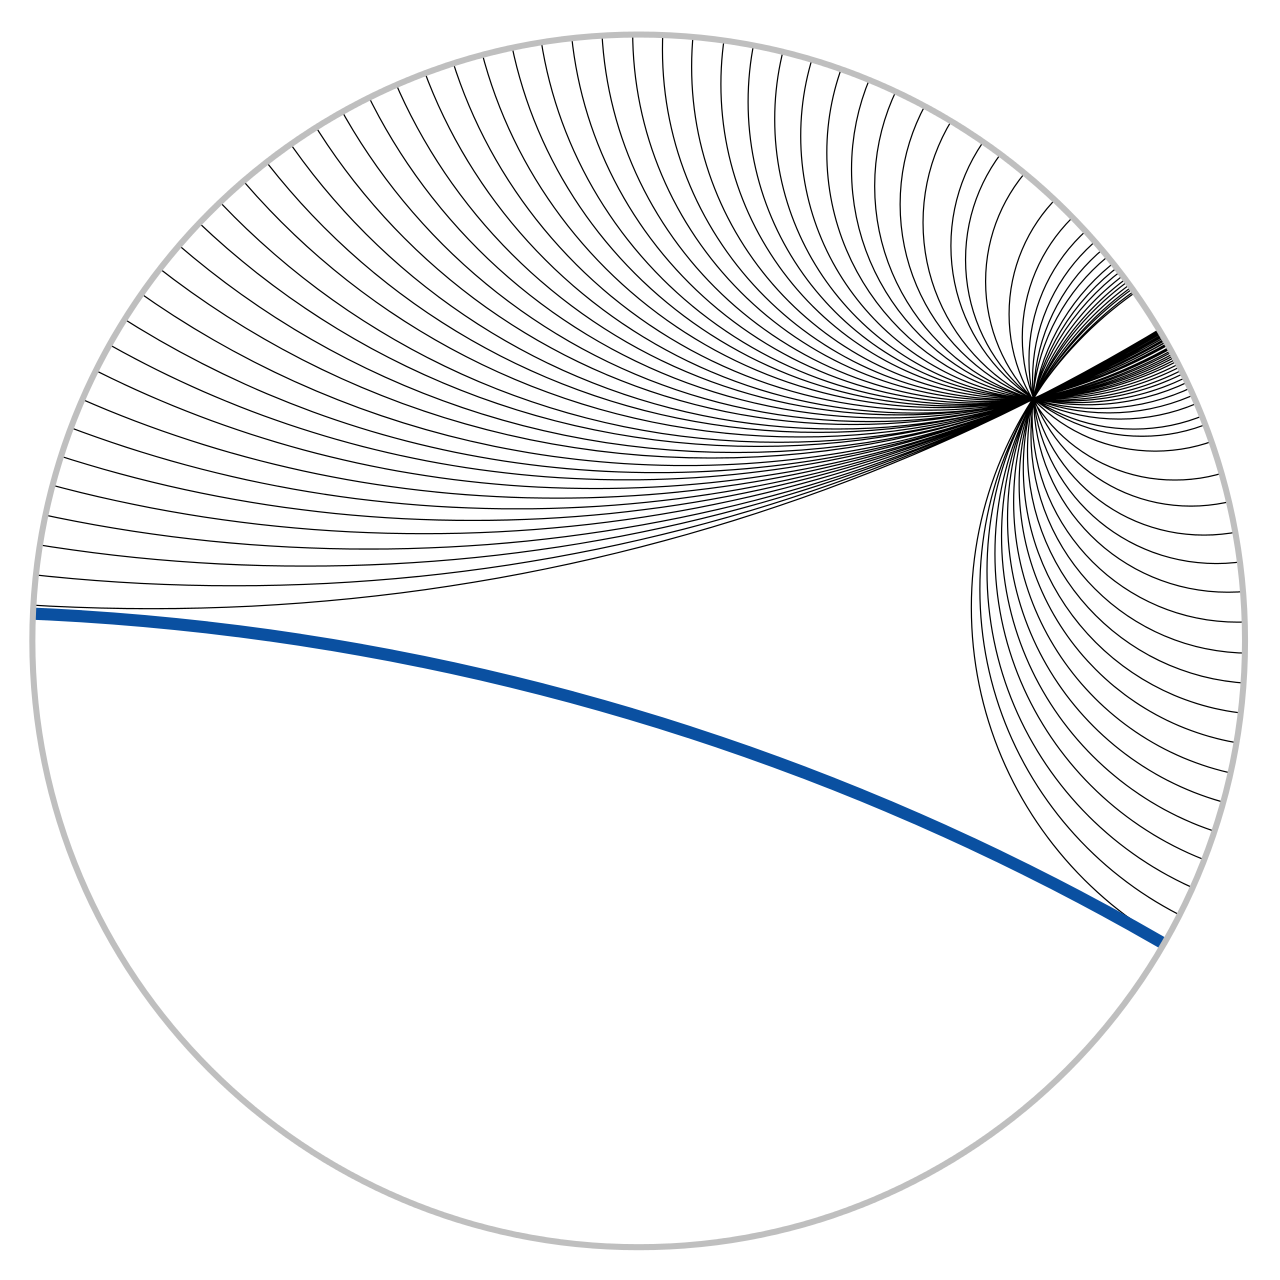
\includegraphics[width=5.5cm]{./imgs/Poincare_disc_hyperbolic_parallel_lines.png}}
	\caption*{En el disco de Poincaré existen infinitas líneas paralelas a una
		dada que pasan por un punto fijo.}
	\label{figure:poincare}
\end{figure}

Podríamos considerar estos modelos y formalizar sus construcciones en \textit{}.
Para ello habría que definir los tipos \textit{Line} y \textit{Point}, las
distintas relaciones de incidencia, orden y congruencia para estos tipos,
demostrar que se cumplen los axiomas de los planos de Hilbert pero no el de las
paralelas. Esto se puede hacer precisamente mediante el mecanismo de las
instancias de clases.








\section{Conclusiones}

- No todo el trabajo está en Lean. A veces no es inmediato cómo formalizar una
proposición en Lean. Hay que tener claros los conceptos y conocer muy bien qué es lo que se
está formalizando.

- Enunciados aparente muy simples pueden ser difíciles y largos de demostrar.

- No se ha pretendido alcanzar una síntesis y claridad en las demostraciones,
sino conseguir que el sistema las acepte. Probablemente muchos de los resultados
pueden ser

- Lean es muy avanzado y en diversas ocasiones nos hemos encontrado con errores
o comportamientos que no hemos sabido interpretar, debido a

- Las mayores dificultades han surgido a la hora de intentar formalizar ejemplos
concretos, como modelos de los distintos grupos de axiomas que se consideran.
Por ejemplo no he conseguido terminar de formalizar el modelo más simple que he
encontrado de una geometría de incidencia en el que no se cumple el axioma de
las paralelas.

En parte atribuyo estas dificultades a la falta de una documentación más
accesible de la librería \textit{mathlib} y cómo están implementados ciertos
objetos matemáticos en ella.

Para usar Lean a un nivel un poco más avanzado que el de este trabajo es
inevitable entrar en ciertos detalles de la teoría de tipos \textit{Calculus of
	Inductive Constructions} y cómo está implementada en \textit{Lean}.


\todo{Redactar}




\appendix
\section{Repositorio de código}\label{sec:repositorio}


\section{Entorno de desarrollo}\label{sec:entorno}

\subsection*{Visual Studio Code}

El entorno recomendado\footnote{Lean también tiene soporte mediante plugins para
	los editores \textit{emacs} y \textit{vim}.} para desarrollar código
\textit{Lean} es el editor \textit{Visual Studio Code}\footnote{Aconsejamos
	utilizar la distribución de \textit{Visual Studio Code} de software libre,
	\href{https://vscodium.com/}{VSCodium}.}. En este editor, una vez instalado el
plugin que da soporte a \textit{Lean}, tenemos acceso a una serie de
herramientas que facilitan la lectura y desarrollo de código en Lean. A
continuación exponemos alguna de estas herramientas.

\subsection*{Consulta de tipos}

Moviendo el cursor por encima de definiciones o tácticas podemos obtener
información adicional sobre un término, tipo o táctica, accediendo a su tipo, su
definición o la documentación correspondiente.

\subsection*{Símbolos matemáticos}

Como se ha mencionado anteriormente en este documento, en \textit{Lean} se
pueden utilizar símbolos unicode para expresar tipos útiles en la formalización
de matemáticas y obtener así un código más cercano a las notaciones lógicas a
las que estamos acostumbrados a usar en matemáticas.

La inclusión de estos caracteres está facilitada en el entorno de desarrollo,
escribiendo comandos que empiecen por \texttt{\textbackslash} estos se
reemplazarán por el caracter correspondiente. Por ejemplo al escribir
\texttt{\textbackslash to} este comando se reemplazará automáticamente por el
caracter \lstinline{→}, \texttt{\textbackslash lambda} por \lstinline{λ} y
\texttt{\textbackslash N} por \lstinline{ℕ}. Si mantenemos el cursor encima de
un símbolo, un panel informativo nos indicará el código que podemos utilizar
para escribirlo.

\subsection*{Panel de estado táctico}

La herramienta más importante de este entorno es el panel lateral desde el cual
podemos consultar el estado táctico. En la siguiente captura de pantalla se ve
cómo, situando el cursor en un paso de una demostración, el panel lateral
proporciona toda la información contextual del estado táctico correspondiente.

\begin{figure}[htbp]
	\centerline{\frame{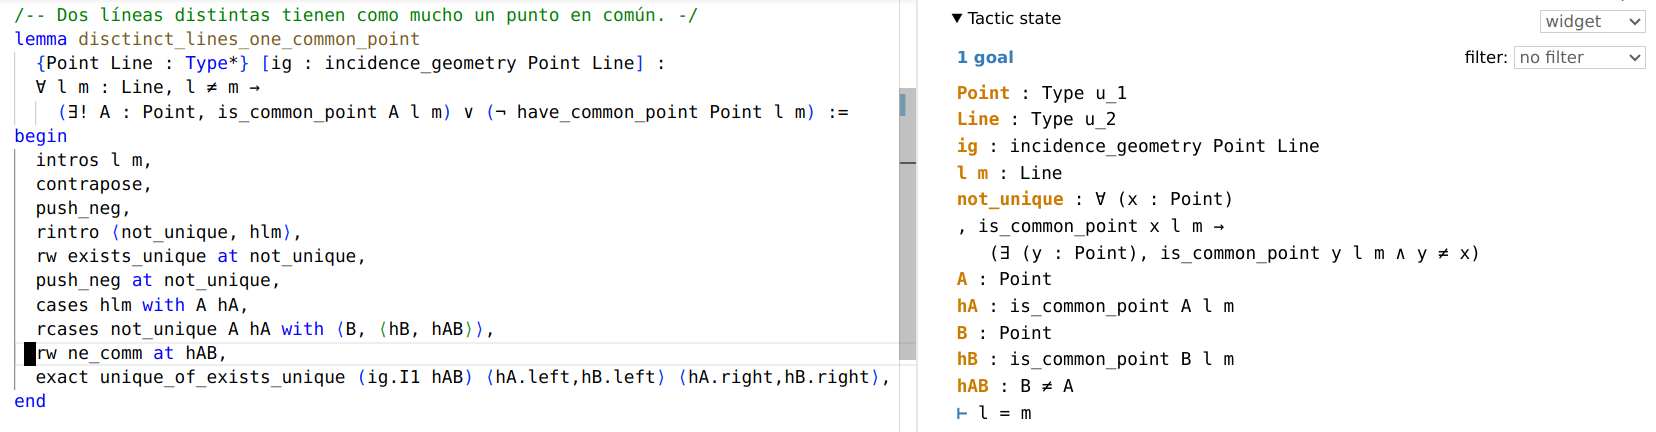
\includegraphics[width=17cm]{./imgs/captura.png}}}
	\caption*{Captura de pantalla del entorno de dearrollo en el editor \textit{Visual Studio Code}.}
	\label{figure:entorno}
\end{figure}

Durante la formalización o lectura de una demostración en \textit{Lean} estamos
continuamente moviéndonos a través del código y observando de qué forma varía el
estado táctico.




\newpage
\printbibliography[heading=bibintoc, title={Referencias}]

\end{document}





